\section{Durchführung}
\label{sec:Durchführung}

\section{Implementation}
\label{sec:implementation}
This experiment uses a diode laser as a source of coherent light. The light can be adjusted by a turning a screw that changes the angle of a diffraction grating. 
<<<<<<< HEAD
In addition to that, a so called collimator is used to narrow the emitted light to a smaller, more precise beam. 
||||||| 9e02252
In addition to that, a so called collimator is used to narrow the emitted light to a smaller, more precise beam 
=======
In addition to that, a so called collimator is used to narrow the emitted light to a smaller, more precise beam  
>>>>>>> 19517064367b79a73aa0318d2aa0ca8c56f141ee


\subsection{Rubidium Flourescence and its spectrum}
\label{sec:Rubi}
For the study of Rubidium's Flourescence, the experiment used for the first part of this experiment needs to be modified.
The Rubidium Cell, which is placed between Field Coils and inside a heater to control its temperature, is set up between the ND Filter Holder and the laser.

\begin{wrapfigure}{r}{0.32\textwidth}
    \begin{center}
        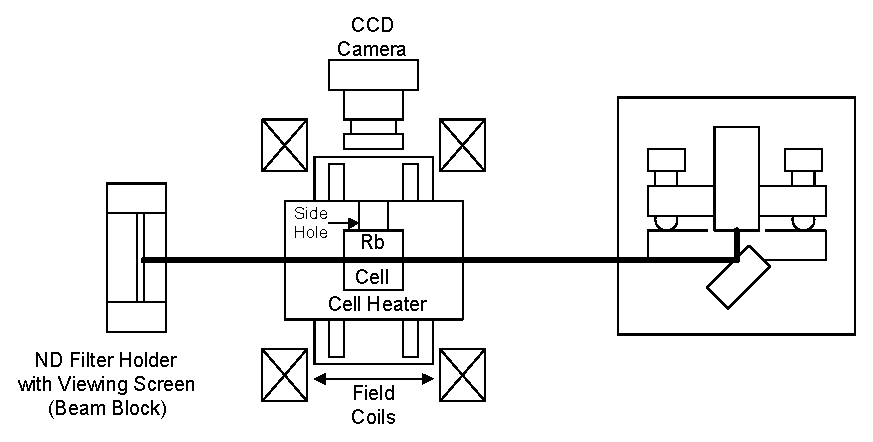
\includegraphics[width=0.3\textwidth]{Setup2.png}
        \caption{Setup for \cite{ap60}.}
        \label{fig:Setup2}
    \end{center} 
\end{wrapfigure}